% !TeX program = platex_custom
\documentclass[twocolumn,a4j]{jsarticle}
\usepackage[top=15truemm,bottom=20truemm,left=20truemm,right=20truemm]{geometry}
\usepackage{amsmath}
\usepackage{amsfonts}
\usepackage{amssymb}
\usepackage[dvipdfmx]{graphicx}
\usepackage[hang,small,bf]{caption}
\usepackage[subrefformat=parens]{subcaption}
\usepackage[dvipdfmx]{color}
\usepackage{listings}
\usepackage{listings,jvlisting}
\usepackage{framed}
\usepackage[dvipdfmx]{hyperref}
\usepackage{ascmac}
\usepackage{enumerate}
\usepackage{tabularx}
\usepackage{cancel}
\usepackage{scalefnt}
\usepackage{overcite}
\usepackage{otf}
\usepackage{multicol}
\usepackage[geometry]{ifsym}
\usepackage{array}

\renewcommand{\figurename}{Fig.}
\renewcommand{\tablename}{Table }

\lstset{
basicstyle={\ttfamily},
identifierstyle={\small},
commentstyle={\smallitshape},
keywordstyle={\small\bfseries},
ndkeywordstyle={\small},
stringstyle={\small\ttfamily},
frame={tb},
breaklines=true,
columns=[l]{fullflexible},
xrightmargin=0zw,
xleftmargin=3zw,
numberstyle={\scriptsize},
stepnumber=1,
numbersep=1zw,
lineskip=-0.5ex
}

% キャプション後ろのダブルコロンを消す
\makeatletter
\long\def\@makecaption#1#2{%
  \vskip\abovecaptionskip
  \iftdir\sbox\@tempboxa{#1\hskip1zw#2}%
    \else\sbox\@tempboxa{#1 #2}%
  \fi
  \ifdim \wd\@tempboxa >\hsize
    \iftdir #1\hskip1zw#2\relax\par
      \else #1 #2\relax\par\fi
  \else
    \global \@minipagefalse
    \hbox to\hsize{\hfil\box\@tempboxa\hfil}%
  \fi
  \vskip\belowcaptionskip}
\makeatother

% タイトル
\makeatletter
\def\@maketitle
{
\begin{center}
{\LARGE \@title \par}
\end{center}
\begin{flushright}
{\large \@date 報告書 No.42}\\
{\large M2 \@author}
\end{flushright}
\par\vskip 1.5em
}
\makeatother

\author{来代 勝胤}
\title{令和5年度 1月 第3週 報告書}
\date{2024/1/16}

\begin{document}
\columnseprule=0.1mm
\maketitle

\section{数値シミュレーションによる性能評価}
\subsection{一様流}

\subsubsection*{改善点}
\begin{itemize}
  \item \textgt{粒子位置計算プログラムの修正}
  \item \textgt{レーザーシートの厚み変更:青色を 1.5 mm に変更}
\end{itemize}

$\blacksquare$ \textgt{流れ場}
\begin{align*}
  (u, v, w) & = (250, 0, 0) \;\rm{[mm/s]}
\end{align*}

$\blacksquare$ \textgt{シミュレーション時間}
\begin{align*}
  t & = 5.5 \;\rm{[s]}
\end{align*}

$\blacksquare$ \textgt{粒子数密度}
\begin{table}[hbtp]
  \centering
  \caption{Particle density}
  \begin{tabular}{c c c c}
    \hline
    Case 1 & $n = 3.0 \times 10^6$ & [$-/\rm{m}$] \\ \hline
    Case 2 & $n = 3.0 \times 10^7$ & [$-/\rm{m}$] \\ \hline
    Case 3 & $n = 3.0 \times 10^8$ & [$-/\rm{m}$] \\ \hline
    Case 4 & $n = 1.0 \times 10^7$ & [$-/\rm{m}$] \\ \hline
    Case 5 & $n = 2.0 \times 10^7$ & [$-/\rm{m}$] \\ \hline
  \end{tabular}\\
\end{table}

$\blacksquare$ \textgt{解析結果}
\begin{figure}[htbp]
  \centering
  {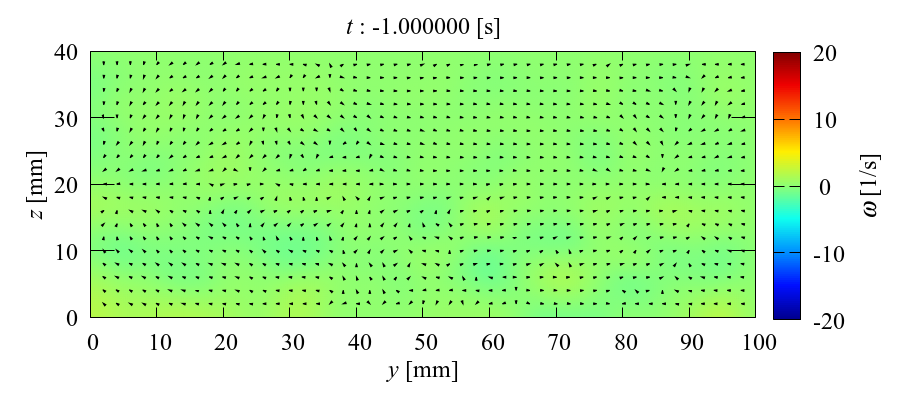
\includegraphics[keepaspectratio, width=80mm]{../images/uniform/velocity_and_vorticity}
    \subcaption{Velocity and vorticity}
    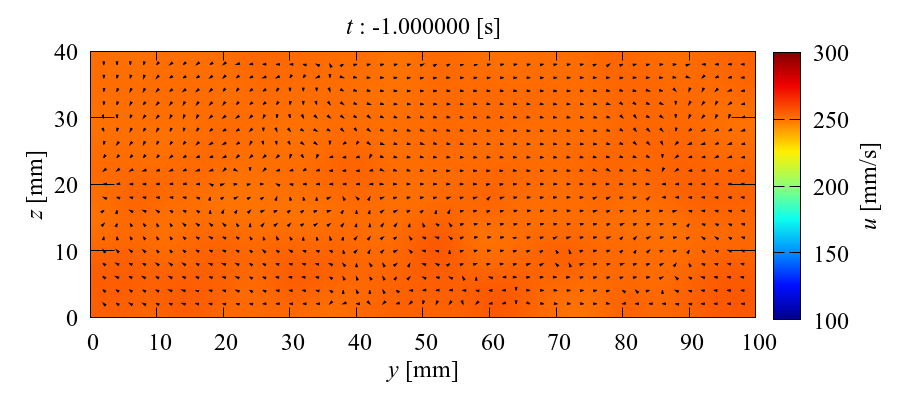
\includegraphics[keepaspectratio, width=80mm]{../images/uniform/velocity_xyz}
    \subcaption{Velocity}
  }
  \caption{Calibrated image}
\end{figure}

\newpage
\subsection{数値評価}

$\blacksquare$ \textgt{RMSE}
\begin{table}[hbtp]
  \centering
  \caption{RMSE of velocity}
  \begin{tabular}{c c c c}
    \hline
           & RMSE:$u$ & RMSE:$v$ & RMSE:$w$ \\ \hline
    Case 1 & 3.961    & 4.562    & 1.255    \\ \hline
    Case 2 & 2.030    & 3.182    & 1.253    \\ \hline
    Case 3 & 29.82    & 30.70    & 1.138    \\ \hline
    Case 4 & 3.052    & 3.790    & 1.219    \\ \hline
    Case 5 & 2.601    & 3.502    & 1.263    \\ \hline
  \end{tabular}\\
\end{table}

ただし,$u, v, w$ は $x, y, z$ 方向の速度成分である.\\
※ 単位は [mm/s] \\

$\blacksquare$ \textgt{予測される誤差量について}

これまでの数値シミュレーションより,
粒子位置の検出および空間校正による$y-z$平面内の誤差は
およそ 0.2 pixel であることがわかっている.
また,粒子クラスタの生成の際に連なる粒子の数は1つ分の変動を持つことがわかっている.
例えば,厚み $T=3 \rm{mm}$ のレーザーシートを主流速度 $u=250 \rm{mm/s}$ で通過する粒子を
フレームレート$f=800 \rm{fps}$ で撮影するとする.
そのとき,粒子がレーザーシートを通過するフレーム数を $\Delta n$ とすると,
\begin{align*}
  \Delta n & = \frac{T}{u} \times f = \frac{3}{250} \times 800 = 9.6
\end{align*}
とあらわせる.
すなわち,実際に粒子を撮影する場合,
粒子クラスタは8および9個の粒子が撮影されるからである.
そして,粒子クラスタには長いクラスタ $n_l$ と短いクラスタ $n_s$ が存在することがわかる.
このとき,粒子クラスタのマッチングによる組み合わせは以下の4パターンが考えられる.

\begin{table}[hbtp]
  \centering
  \caption{Pair of particle clusters}
  \begin{tabular}{c c c c}
    \hline
    (1) & $n_{1s}$ & $n_{2s}$ & フレーム差は正しく計算  \\ \hline
    (2) & $n_{1s}$ & $n_{2l}$ & フレーム差は0.5枚分増加 \\ \hline
    (3) & $n_{1l}$ & $n_{2s}$ & フレーム差は0.5枚分増加 \\ \hline
    (4) & $n_{1l}$ & $n_{2l}$ & フレーム差は正しく計算  \\ \hline
  \end{tabular}\\
  \vskip 0.2 \baselineskip
  ※ 添え字はレーザーシートの番号を表す.
\end{table}

したがって,粒子クラスタのマッチングによるフレーム差の誤差 $\delta n$ は
\begin{align*}
  \delta n & = +0.5
\end{align*}
となる.

また,粒子が1フレームごとに画像内を移動する距離は $y$方向に
4 [pixel],$z$方向に 0 [pixel] 程度であることがわかっている.
すなわち,マッチングした粒子クラスタ中心がそれぞれ $\pm 0.2$ pixel,
マッチング時に生じるフレーム差の誤差 $\delta n$ によって
$y$方向に$4 \times \delta n = +2$ pixel の誤差が生じると考えられる.
したがって,マッチング時に生じる$y$方向誤差 $\delta e_y$,$z$方向誤差 $\delta e_z$ は
\begin{align*}
  \delta e_y & = 2 \pm 0.2 \;\rm{[pixel]} \\
  \delta e_z & = \pm 0.2 \;\rm{[pixel]}
\end{align*}
ここで,画像サイズと撮影範囲の比率を $\alpha$ とすると,
画像の横幅 $w = 800 \rm{pixel}$,撮影範囲の横幅 $W = 100 \rm{mm}$ であるから,
\begin{align*}
  \alpha & = \frac{W}{w} = 0.125 \;\rm{[mm/pixel]}
\end{align*}
したがって,マッチング時に生じる誤差 $\delta e_y$,$\delta e_z$ は
\begin{align*}
  \delta e_y & = 2 \pm 0.2  = 0.25 \pm 0.025 \;\rm{[mm]}        \\
  \delta e_z & = \pm 0.2 \;\rm{[pixel]} = \pm 0.025 \;\rm{[mm]}
\end{align*}
とあらわすことができる. 

また,一様流のとき,主流方向速度 $u$ であるため,
レーザーシート間距離 $X$ を通過するのにかかる時刻を $\delta t$ とすると,
\begin{align*}
  \delta t & = \frac{X}{u} = \frac{2.5}{250} = 0.01 \;\rm{[s]}
\end{align*}
したがって,マッチング時に生じる誤差 $\delta e$ から
予測される速度誤差 $\delta u$ は
\begin{align*}
  \delta v & = \frac{\delta e_y}{\delta t} = 25 \pm 2.5 \;\rm{[mm/s]} \\
  \delta w & = \frac{\delta e_z}{\delta t} = \pm 2.5 \;\rm{[mm/s]}
\end{align*}

\newpage
\section{三角翼モデル}
$\blacksquare$ \textgt{数値シミュレーション}
\begin{figure}[htbp]
  \centering
  {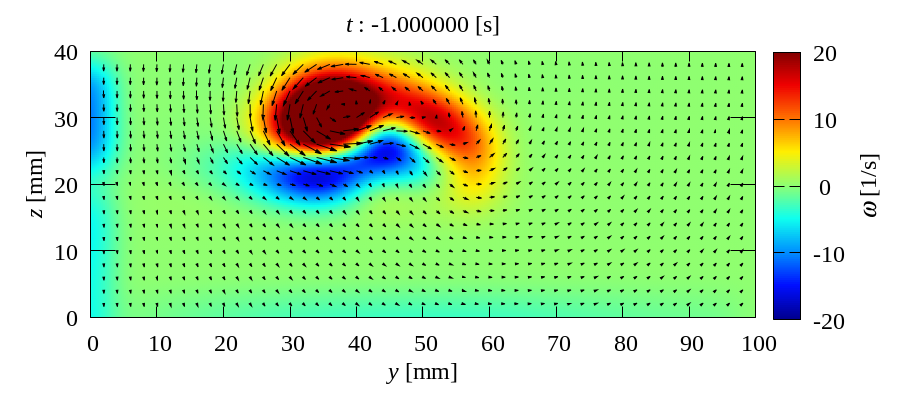
\includegraphics[keepaspectratio, width=80mm]{../images/simulation/velocity_and_vorticity}
    \subcaption{Velocity and vorticity}
    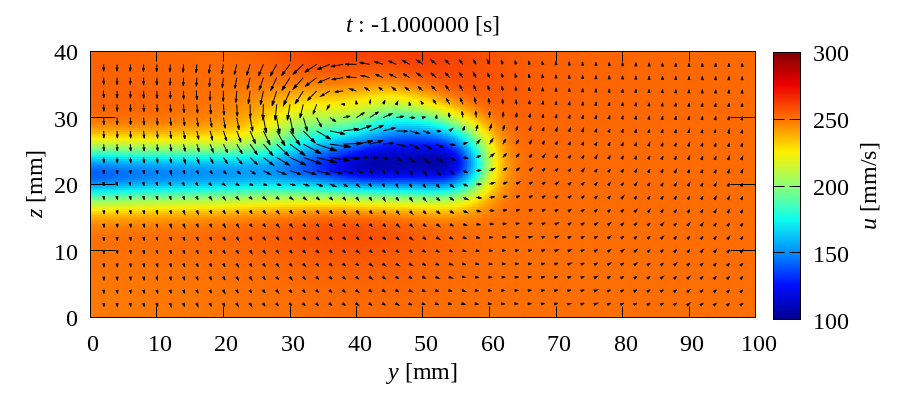
\includegraphics[keepaspectratio, width=80mm]{../images/simulation/velocity_xyz}
    \subcaption{Velocity}
  }
  \caption{Delta wing : Numerical simulation}
\end{figure}

$\blacksquare$ \textgt{解析結果}
\begin{figure}[htbp]
  \centering
  {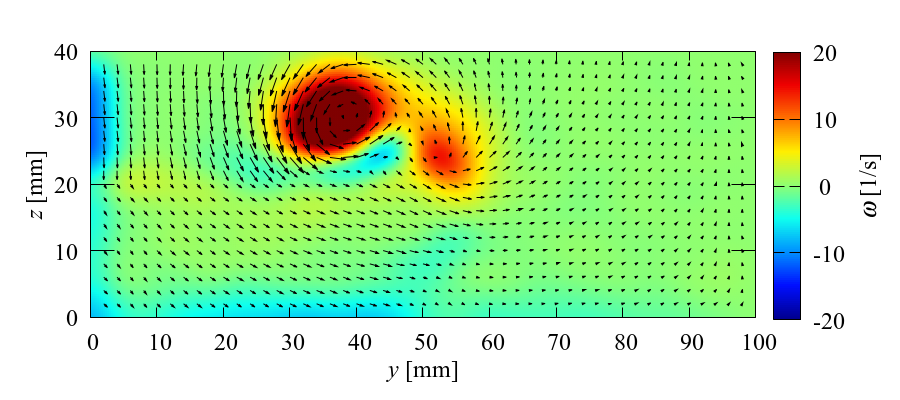
\includegraphics[keepaspectratio, width=80mm]{../images/analysis/velocity_and_vorticity}
    \subcaption{Velocity and vorticity}
    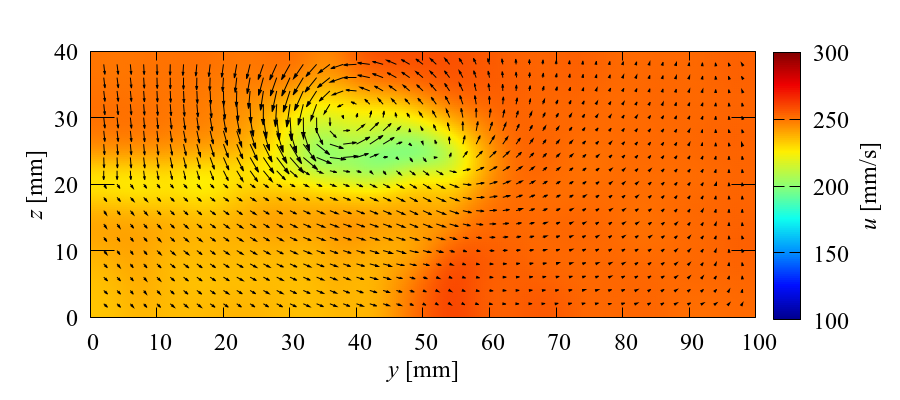
\includegraphics[keepaspectratio, width=80mm]{../images/analysis/velocity_xyz}
    \subcaption{Delta wing : Analysis}
  }
  \caption{Calibrated image}
\end{figure}

\end{document}